\documentclass{amcs}

\title[Implemention and evaluation...]{Implementation and evaluation of fine-tuning methods of PI controller with PLC-PID Tuner}

\author[ad1][ad2]{Jakub MOŻARYN}
\author[ad1][]{Damian SUSKI}
\author[ad1][ad2]{Arkadiusz WINNICKI}


\correspondingauthor{Second AUTHOR}

\address[ad1]{Institute of Automatic Control and Robotics\\ Warsaw University of Technology, Address ul. Sw. A. Boboli 8, 02-525, Warsaw, Poland\\ e-mail: \url{j.mozaryn@mchtr.pw.edu.pl}}


\Runauthors{F. Author \it{et al.}}
%\Runauthors{J. Doe}
%\Runauthors{J. Doe and M. John}

%PLEASE DO NOT MODIFY OR REMOVE THESE!
%\Year{}
%\Vol{}
%\No{}
%\Startpage{}
%\Endpage{}
%\DOI{}
%\Received{}
%\Revised{}
%\Rerevised{}
%\Accepted{}

\bibliographystyle{dcu}

\begin{document}
\begin{abstract}
In the paper, the method of an iterative modification of tuning parameters of a PI controller is presented. Proposed algorithms base on the off-line evaluation of quality indices. They were tested using PLC-PID Tuner - the application developed for tuning PID controller in S7 Simatic PLCs. It was shown that for some cases  proposed iterative method of modifying tuning parameters might increase the control quality. Furthermore, the gain margin and phase margin achieved  through this method are close to values recommended for  practical applications.
\end{abstract}

\begin{keywords}
keyword 1, keyword 2, \dots, keyword 5. Please provide a few keywords (3--5) and keep them specific.
\end{keywords}
\maketitle

\section{Introduction}
Despite all the progress in advanced control, the PID (proportional-integral-derivative) algorithm remains the most popular. Its gains are often chosen independently by an engineer, based on his experience or through some simple selection methods such as \textit{Ziegler-Nichols} \cite{Ziegler:1942} or \textit{Cohen-Coon} \cite{Cohen:1953}. However, regardless of the type of controlled process, there is usually requirement of exact response of the system. Without proper methodology of controller parameters tunig the quality of the control system may be unsatisfactory. Therefore many scientists and engineers develop tuning rules for different processes, where they consider different objectives. The survey presented in \cite{Odwyer:2006} gives the total of 1134 separate rules for PI and PID controllers. Such statistics were done in 2006, and one can expect that until now this number has increased significantly.

Nowadays, most of small and medium size production lines are controlled by Programmable Logic Controllers (PLC) which allow user to create the simple single loop control system as well as more complex structures. The main issue that ensures the correct functionality of the automation system is a proper adjustment of controller parameters. It should allow to minimize the deviation of the process variables from the desired output response, and therefore reduce the cost of the process due to the energy and material losses. 

In many practical situations, it is impossible to develop one's own tuning rules. Popularity of PLC controllers result in the need to implement appropriate tools that support user during controller tuning. Unlike automation systems based on dedicated controllers such as Distributed Control System (DCS), solutions based on PLC don't have such wide support in terms of integration and operation of control algorithms. 

Recently, manufacturers of automation systems develop advanced software tools that allow autotuning of PID controllers implemented in PLC's, using  proprietary algorithms based on relay or area auto-tuning methods \cite{Astrom:1995}, \cite{Yu:2006}, \cite{Trybus:2011}. Such modules which facilitate PID tuning are integrated within e.g. TIA Portal (Siemens), Automation Studio (B\&R) or TwinCAT (Beckhoff) software. However, implemented  methods don't allow designing control system in terms of specific performance indexes \cite{Bishop:2010}, \cite{Mozaryn:2013} e.g. gain and phase margin, integral of the squared error (ISE) or the integral of the absolute value of error (IAE). Therefore, it has limited use in processes which apart from minimizing standard indices, must meet additional criteria like sensitivity or robustness. 

Most applications that allow identification (e.g. IDCAD \cite{Janiszowski:2002}, MATLAB/Simulink, LabVIEW) don't have automatic procedures for tuning the specific controller, especially in industrial environment where the additional software is required to communicate with PLC to collect and archive values of the process variables. After process identification, controller parameters can be calculated   \cite{Odwyer:2009} and then implemented in PLC. Based on these premises the choice of proper method in industrial environment can be very complicated and time consuming. Therefore, the possibility to test, compare and use of wide variety of methods is very reduced. 

These facts were the inspiration to create PLC-PIDTuner application which combines above mentioned functionalities: real process data collection using Simatic S7 1200/1500 controllers, SISO system identification, tuning of PID controller parameters with different methods, verification of the control system in time and frequency domains using various performance indices. PLC-PIDTuner simplifies the tuning rule selection process and can be used by the field engineers with basic knowledge of control engineering.

The article is organized as follows. In section II, the implementation details of PLC-PIDTuner are described. Then, in section III, the PLC controller tuning methodology is presented. Section IV describes results obtained during exemplary verification of developed application, based on a model of the 3rd order lag system with delay. Finally, in section V further development ideas are presented and in section VI concluding remarks are given..

\section{Title page}
The title area is created using the \verb+\maketitle+ command. Before invoking this command, the author has to declare all objects required to appear in the title area.

\subsection{Manuscript title}
\label{title}
An example title is declared as follows:

\medskip
\noindent {\small \verb+\title{Numerical analysis of the algorithm}+}.

\medskip\noindent
The title is used to format the headers of odd pages. The header of each odd page is left justified and the page number right justified. In the case of a very long title, please use its short version, e.g., the first few words of the title and an ellipsis. The authors can put the short title of the paper in square brackets as an optional parameter of the \verb+\title+ command, e.g.,

\medskip
\noindent {\small \verb+\title[Numerical analysis ...]{Numerical+} {\small \verb+analysis of the algorithm}+}.

\subsection{Authors' names and affiliations}
The authors' names and affiliations are declared with two types of commands. By default, \verb+\author+ along with \verb+\address+ is used. Here, each author can be assigned at most two institutions:

\medskip
\noindent {\small \verb+\author[ad1][ad2]{Author's NAME}+}.

\medskip\noindent
If an author is assigned one institution only, the second square brackets should be empty:

\medskip
\noindent {\small \verb+\author[ad1][]{Author's NAME}+}.

\medskip\noindent
For each author, a separate \verb+\author+ command should be run, e.g.,

\medskip
\noindent {\small \verb+\author[ad1][]{First Author's NAME}+}
\noindent {\small \verb+\author[ad2][]{Second Author's NAME}+}.

\medskip\noindent
\emph{Important!} The \verb+\author+ command permits to declare at most six authors.

To define an author's affiliation, the \verb+\address+ command can be used:

\medskip
\noindent {\small \verb+\address[ad1]{First affiliation}+}.

\medskip\noindent
The option in square brackets is mandatory in order to assign an author to this institution. For each institution, a separate \verb+\address+ command should be run, e.g.,

\medskip
\noindent {\small \verb+\address[ad1]{First affiliation}+}
\noindent {\small \verb+\address[ad2]{Second affiliation}+}.

\medskip\noindent
\emph{Important!} The \verb+address+ command permits to declare at most six institutions.

Please note that the corresponding author for the paper must be marked as

\medskip
\noindent {\small \verb+\correspondingauthor{Author's NAME}+}.

\medskip\noindent
Another option is \verb+\authors+ along with  \verb+\addresses+. These may be used \textbf{only} for more than six authors or more than two institutions per author. Please note that here care must be taken while associating given symbols with names, and these must be Latin lower case characters. Here the corresponding author is marked with the \verb+\thanks+ command, as exemplified in the commented preamble passage above.

Note that in all cases at least one institution must be declared for each author!

\medskip\noindent
\emph{Important!} The corresponding author should be chosen carefully---his or her task will include contact and cooperation with the Editorial Office, representing the co-authors and ensuring communication between all parties involved.

\subsection{Abstract and keywords}
The abstract text is encapsulated within the \verb+abstract+ environment:

{\small \begin{verbatim}
\begin{abstract}
The paper deals with ...
\end{abstract}.
\end{verbatim}}

\noindent The list of keywords is defined using the \verb+keywords+ environment:

{\small \begin{verbatim}
\begin{keywords}
keyword1, keyword2, keyword3 ...
\end{keywords}.
\end{verbatim}}

\subsection{Header of the title page}
The header of the title page contains the name of the journal and the following information:
\begin{itemize}
  \item
    Publication year, declared with the \verb+\Year{}+ command;
  \item
    Journal volume number, declared with the \verb+\Vol{}+ command;
  \item
    Journal issue number, declared with the \verb+\No{}+ command;
  \item
    Paper final page numbering, declared with the \verb+\Startpage{}+ and \verb+Endpage{}+ commands, respectively;
  \item
    Digital Object Identifier number, declared with the \verb+DOI{}+ command.
\end{itemize}
These commands are used solely by the editorial staff, so the authors are asked to ignore them.

\section{Headers}
The header of each even page includes names and initials as well as the page number. To declare the authors' names, please use the \verb+\Runauthors{}+ command placed in the document preamble (before \verb+maketitle+). For one author, give the first name initial and the full last name, e.g., for John Doe, the appropriate form is

\medskip\noindent {\small \verb+\Runauthors{J. Doe}+}.

\medskip\noindent
For two authors, use both authors' names, e.g.,

\medskip\noindent {\small \verb+\Runauthors{J. Doe and M. John}+}.

\medskip\noindent For more than two authors, use the first author's name and ``\emph{et al.}'', e.g.,

\medskip\noindent {\small \verb+\Runauthors{J. Doe \it{et al.}}+}.

\medskip The header of each odd page contains the title of the paper and the page number. To declare the header of each odd page, please use the {\small \verb+\title+} command (see Section~\ref{title}).

\section{Sections}
Sections are defined in a common way by the commands \verb+\section+, \verb+\subsection+, \verb+\subsubsection+ and \verb+\paragraph+. Arabic numbers are used for subsequent numbering. A paragraph is a section without a number. Below are examples of section formatting:

\subsection{Secondary heading} Section text.
\subsubsection{Tertiary heading} Section text.
\paragraph{Paragraph} Section text.

\section{Floating material}
%
\begin{figure}[!b]
 \centering
  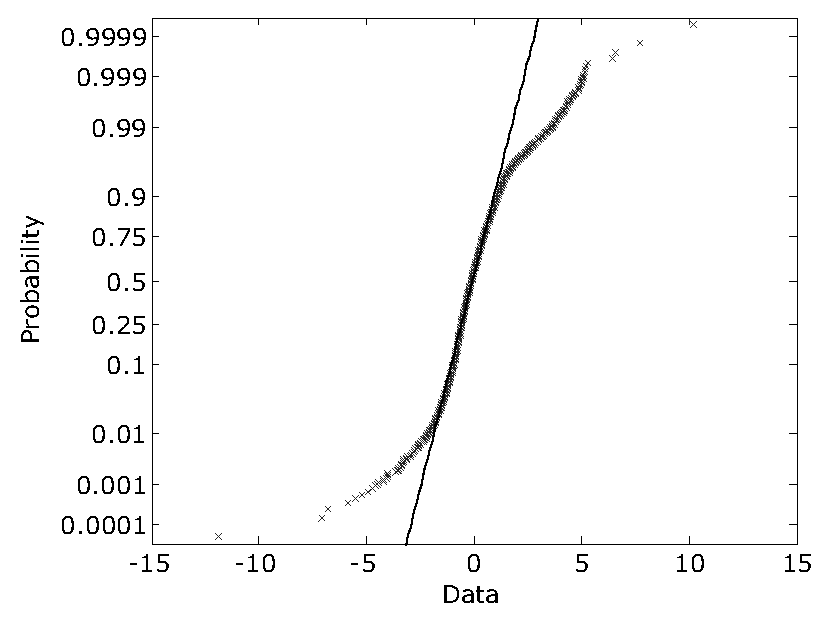
\includegraphics[width=0.45\textwidth]{fig1}
 \caption{Figure example \protect \cite{Haykin:99}.}
  \label{fig1}
\end{figure}
%
\begin{figure*}[!t]
 \centering
  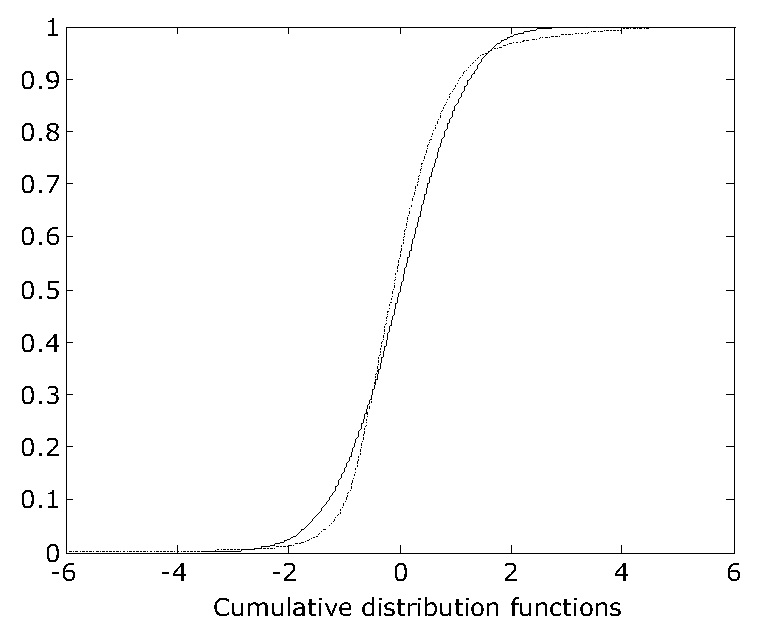
\includegraphics[width=0.40\textwidth]{fig2a}\hspace{0.5cm}
  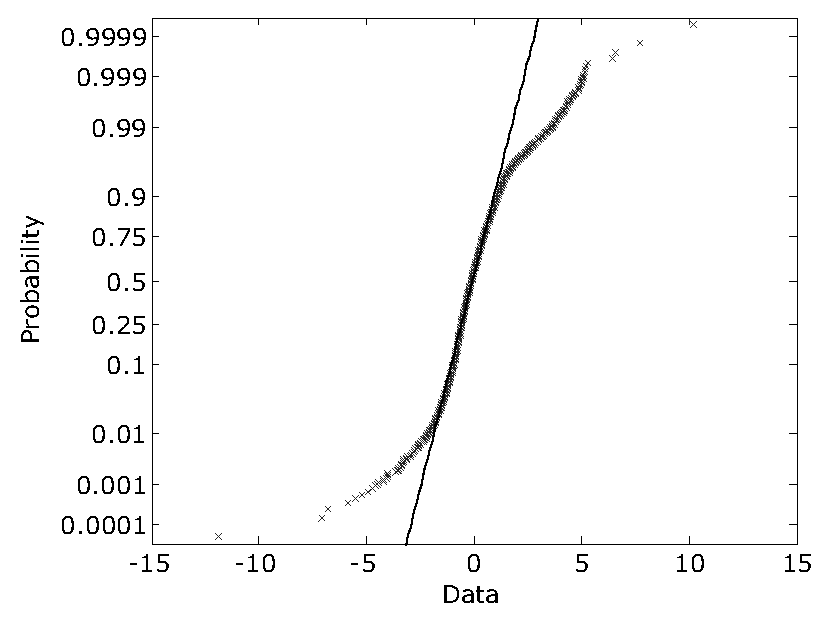
\includegraphics[width=0.45\textwidth]{fig2b}\\
  (a)\hspace{8cm}(b)
  \caption{Sample figure: the first graph (a), the second graph (b).}
  \label{fig2}
\end{figure*}
%
\subsection{Figures}
Figures are defined in a standard manner, e.g.,
{\small \begin{verbatim}
\begin{figure}[!b]
 \centering
 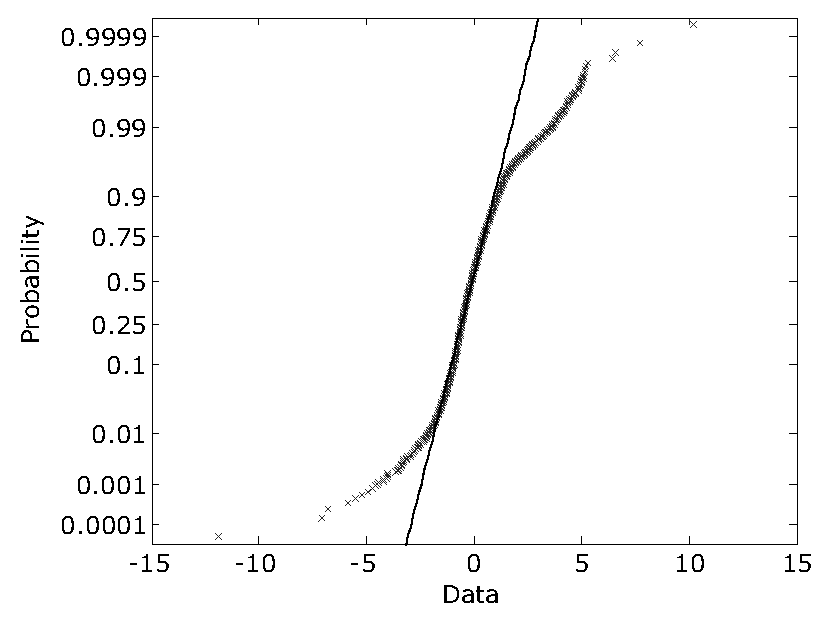
\includegraphics[width=0.45\textwidth]
 {fig1}
 \caption{Figure example.}
 \label{fig1}
\end{figure}.
\end{verbatim}}
\noindent They should be centred and placed at the top or bottom of a page if possible, as close as possible to the first reference to them. Please avoid middle in-text placement (option \verb+h+), and do not introduce frames around the figures. To use the \verb+\includegraphics+ command, the \verb+graphicx+ package has to be loaded first. The caption of a figure is placed below the figure to which it refers and should be ended with a full stop. In the case of multiple-part figures, enumerate each piece as (a), (b), etc., including necessary descriptions in the main caption of the figure. Use the \verb+caption+ command with the \verb+caption2+ package to format figure captions. Make sure you always employ \LaTeX commands for figure captions and numbering instead of incorporating those into the original graphics.

Sometimes figures are too wide to fit in a single column. Then, a double-column figure environment declared with the \verb+figure*+ environment can be used:
%
{\small \begin{verbatim}
\begin{figure*}[!t]
 \centering
 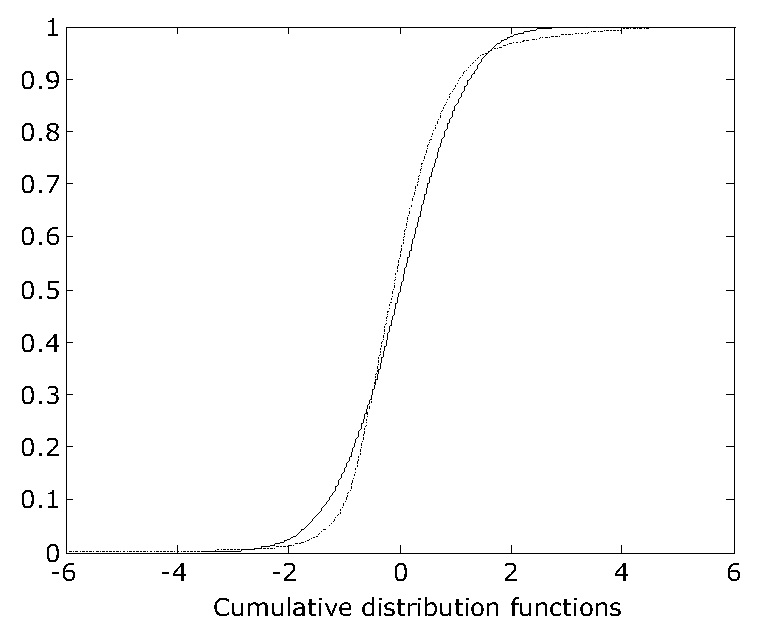
\includegraphics[width=0.405\textwidth]
 {fig2a}\hspace{0.5cm}
 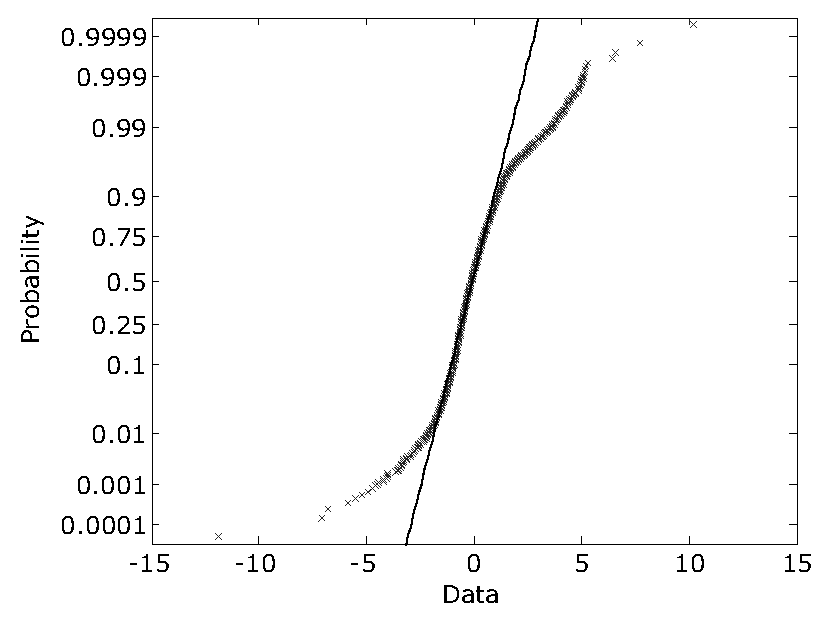
\includegraphics[width=0.45\textwidth]
 {fig2b}\\
 (a)\hspace{7cm}(b)
 \caption{Sample figure: the first
 graph (a), the second graph (b).}
 \label{fig2}
\end{figure*}.
\end{verbatim}}

When referring to figures, the abbreviation ``Fig.'' should be used. It is also advisable to clearly name the graphic files and their labels, e.g., \emph{fig1, fig2a, fig2b}, etc.
\subsection{Tables}
%
Tables should be centred, at the top or bottom of a page if possible, and as close as possible to the first reference to them. The caption of a table should be placed over the table to which it refers and should be ended with a full stop. For example, the code
%
{\small\begin{verbatim}
\begin{table}[!b]
 \centering
 \caption{Table example.}
 \label{table1}
 \begin{tabular}{|c|c|c|}
  \hline
  Algorithm & Performance [\%]& Calc. time
  [s]\\\hline\hline
  gradient & 95 & 100\\
  stochastic & 97 & 80\\
  evolutionary & 99 & 500\\\hline
 \end{tabular}
\end{table}
\end{verbatim}}
\noindent refers to Table~\ref{table1}. For long tables, please use the \verb+table*+ environment.
%
\begin{table}[!b]
 \centering
 \caption{Table example.}
 \label{table1}
 \begin{tabular}{|c|c|c|}
   \hline
   Algorithm & Performance [\%]& Calc. time [s]\\\hline\hline
   gradient & 95 & 100\\
   stochastic & 97 & 80\\
   evolutionary & 99 & 500\\\hline
 \end{tabular}
\end{table}

\section{Graphics}
Graphics should be composed \textbf{in vector format as gray scale} encapsulated postscript (EPS) or portable document format (PDF) files. Vector images allow good reproduction of graphics both online and in print, are not affected by resizing and take up little space. Therefore, line drawings should be originally composed as vector graphics, while mixed/photographics images may be exported to the EPS/PDF format with the resolution of at least 300 dpi. Please note that we will not be able to drastically improve graphics that are originally of low quality, so the authors are expected to ensure the best possible graphical presentation of their results. (Blurred, pixelated or scanned images will not be accepted!)

Any text used in the images should be converted to curves or composed using embedded PostScript Type 1 fonts---this will ensure correct displaying of the figures in the final PDF file. Please do NOT use the \verb+psfrag+ option in your graphics---instead, incorporate all descriptions into the actual image.

\emph{Important!} As \emph{AMSC} is entirely a monochrome publication, the provided graphics must be in gray scale---any images submitted in colour will be converted to such. Consequently, no in-text references to colour in graphics are allowed. (If needed, readers may be provided with colour graphics via links or contact with the authors---a proper notification should be included in the paper.) Also, please make sure that any fine line drawings such as graphs are legible in gray scale---use fairly thick lines, contrasting shades of gray or symbols.

Be aware that figures, along with abstracts, keywords and tables, often make a first impression about the entire paper, so please make them informative and clean.

\section{Equations}
Equations may be typeset with traditional commands such as \verb+\equation+, \verb+\eqnarray+, etc., but the use of the \verb+\amsmath+ and \verb+\amssymb+ packages is recommended. Each equation should be centred and numbered consecutively, starting from 1. Use arabic numbering in brackets, right justified. Please add (if appropriate) punctuation marks at the end of the formulae, e.g.,
%
\begin{equation}
  J=\sum_{i=1}^N(e_i-y_i^s)^2.
\end{equation}

\noindent \emph{Important!} Please avoid double-column equations.

\section{Theorems and other environments}
The \verb+amcs+ document class offers a number of environments to declare theorems and related structures.

\subsection{Theorems, corollaries, propositions and lemmas} The following piece of code:

{\small \begin{verbatim}
\begin{theorem}{Reference}
 Theorem definition xxxxx xxxx xxx xxx xxx
 xxx xxx xxx xxx xx xx xxxx xxx xxxxx xxxx.
 \label{theorem1}
\end{theorem}
\end{verbatim}}
\noindent results in Theorem~\ref{theorem1}, where reference to a suitable work is given in the brackets.

\medskip
\begin{theorem}{Werbos, 1974}
Theorem definition xxxxx xxxx xxx xxx xxx
xxx xxx xxx xxx xx xx xxxx xxx xxxxx xxxx.
 \label{theorem1}
\end{theorem}

\medskip\noindent
When referencing is not needed, please leave the curly brackets empty, e.g.,
{\small \begin{verbatim}
\begin{theorem}{}
 Theorem definition xxxxx xxxx xxx xxx xxx
 xxx xxx xxx xxx xx xx xxxx xxx xxxxx xxxx.
 \label{theorem2}
\end{theorem}.
\end{verbatim}}

\noindent
The result of the above is as follows:

\begin{theorem}{}
 Theorem definition xxxxx xxxx xxx xxx xxx
 xxx xxx xxx xxx xx xx xxxx xxx xxxxx xxxx.
 \label{theorem2}
\end{theorem}

\medskip \noindent

Instead of a reference, a name can be given to the theorem. In much the same way, \verb+lemma+, \verb+corollary+, \verb+statement+ and \verb+proposition+ environments are declared.

\subsection{Proof environment}
Proofs are handled by the environment
{\small \begin{verbatim}
\begin{proof}{Reference/Name}
 Proof of theorem xxx xxx xxx xxx xxx xx xx
 xxx xxx xxx xxx xxxxx xx xx xxxx xx xx xxx
\end{proof},
\end{verbatim}}

\noindent which results in

\begin{proof}{See Uci\'nski, 1999}
 Proof of theorem xxx xxx xxx xxx xxx xx xx
 xxx xxx xxx xxx xxxxx xx xx xxxx xx xx xxx,
\end{proof}

\medskip

\noindent with an optional parameter for a reference or a name, which may be left empty if not needed. The Q.E.D. symbol {\footnotesize $\blacksquare$} is automatically placed at the end of each proof.

\subsection{Example environment}
Examples are declared by the environment
{\small \begin{verbatim}
\begin{example}[]{Stability}
 Let us consider an example ... xxx xxx
 xxx  xxx xxx  xx xx xxx xxx xxx xxx
 xxxx x xx  xx  xxxx xx xx xxx
\end{example},
\end{verbatim}}

\noindent which results in

\begin{example}[]{Stability}
 Let us consider an example ... xxx xxx
 xxx xxx xxx  xx xx xxx xxx xxx xxx xxxx
 x xx xx  xxxx xx xx xxx.
\end{example}

\medskip \noindent The symbol $\blacklozenge$ is automatically placed at the end of each example. If this sign is not required, please put the \texttt{nosign} option in the brackets, i.e.,

{\small \begin{verbatim}
\begin{example}[nosign]{Stability}
 Proof of theorem xxx xxx xxx xxx xxx xx xx
 xxx xxx xxx xxx xxxxx xx xx xxxx xx xx xxx
\end{example}.
\end{verbatim}}

\subsection{Definitions, problems, remarks and others}

The following piece of code:

{\small \begin{verbatim}
\begin{definition}{Definition name}
 Contents of definition xxxxx xxxx xxx xxx
 xxx xxx xxx xxx xx xx xxxx xxx xxxxx xxxx.
 \label{definition1}
\end{definition}
\end{verbatim}}
\noindent results in Definition~\ref{definition1}, with the name of the definition given in the brackets.

\medskip
\begin{definition}{Equivalence rule}
 Contents of definition xxxxx xxxx xxx xxx
 xxx xxx xxx xxx xx xx xxxx xxx xxxxx xxxx.
 \label{definition1}
\end{definition}

\medskip\noindent
When the name is not needed, please leave the curly brackets empty, e.g.,

{\small \begin{verbatim}
\begin{definition}{}
 Let $x(t)$ be ...xxx xxx xxx xxx xxx xx xx
 xxx xxx xxx xxx xxxxx xx xx xxxx xx xx xxx
\end{definition}.
\end{verbatim}}

\noindent Instead of a name, reference to a suitable work can be given in the brackets. In much the same way, \verb+remark+, \verb+observation+, \verb+assumption+, \verb+property+ and \verb+problem+ environments are declared.

\section{Algorithms}
The algorithms should be expressed using the \verb+algorithmic+ and \verb+algorithm+ environments provided by the \verb+algorithmic.sty+ and \verb+algorithm.sty+ packages, respectively. The \verb+algorithmic+ environment allows describing algorithms while the \verb+algorithm+ environment provides a float wrapper for defined algorithms described using the \verb+algorithmic+ one. The following piece of code:
\begin{verbatim}
\begin{algorithm}[!h]
\caption{Selection of the point.}
\begin{algorithmic}[1]
\REQUIRE $d_1,d_2,\psi$
\IF {$d_2 > \psi^2$}
\STATE $a_1:=d_1, a_2:=\psi^2$
\COMMENT{region I}
\ELSIF {$d_1 \geqslant 2\psi$}
\STATE $a_1:=2\psi$, $a_2:=\psi^2$
\COMMENT{region II}
\ENDIF
\RETURN $a_1,a_2$
\COMMENT{Returns coordinates}
\end{algorithmic}
\end{algorithm}
\end{verbatim}
gives the result portrayed below.
\begin{algorithm}[!h]
\caption{Selection of the stationary point.}
\label{a:alg}
\begin{algorithmic}[1]
\REQUIRE $d_1,d_2,\psi$
\IF {$d_2 > \psi^2$}
\STATE $a_1:=d_1, a_2:=\psi^2$
\COMMENT{region I}
\ELSIF {$d_1 \geqslant 2\psi$}
\STATE $a_1:=2\psi$, $a_2:=\psi^2$
\COMMENT{region II}
\ENDIF
\RETURN $a_1,a_2$
\COMMENT{Returns coordinates}
\end{algorithmic}
\end{algorithm}

Algorithms expressed in a step-by-step manner can be defined in the following way:
\begin{verbatim}
\begin{algorithm}[!h]
\caption{Robust model designing.}
\label{a:alg1}
\textbf{Step 1.} Compute the residual
$r=y - y_m$.

\smallskip
\textbf{Step 2.} Collect the data
$\{u_i,r_i\}_{i=1}^{N}$ and identify
an error model using these data.

\smallskip
\textbf{Step 3.} Construct a robust
model.
\end{algorithm},
\end{verbatim}
which gives Algorithm 2.
\begin{algorithm}[!h]
\caption{Robust model designing.}
\label{a:alg1}
\textbf{Step 1.} Compute the residual $r=y - y_m$.

\smallskip
\textbf{Step 2.} Collect the data $\{u_i,r_i\}_{i=1}^{N}$ and identify an error model using these data.

\smallskip
\textbf{Step 3.} Construct a robust model.
\end{algorithm}

Algorithms formatted in a different manner cannot be accepted.

\section{Acknowledgments}
The acknowledgment section is created using the \verb+acknowledgment+ environment:
{\small \begin{verbatim}
\begin{acknowledgment}
 The authors wish to thank ... xx xxx xx x
 xx xx xxx xxx xxx xxx xxxxx xx xx xxxx xx
\end{acknowledgment}.
\end{verbatim}}
Acknowledgments and other unnumbered sections have the title centered.

Please use this section to acknowledge all and any kinds of support your research has obtained.

\section{References}
Authors should provide complete, correct and properly structured references. All data in a reference must be correct and exhaustive. Please cite the full title of a journal or the full name of a conference, not an abbreviation (e.g., not \emph{IEEE Tran.~N.~Networks} but \emph{IEEE Transactions on Neural Networks}, not \emph{ACC 2007} but \emph{American Control Conference 2007}). Journal publications should contain volume and issue numbers as well as the page range. Book chapters must be accompanied with the book title and editors, publisher and publication city, as well as page numbers. Conference publications should include the conference location (city and country) and page numbers. Alternatively, if published in books, they should be structured as book chapter entries described above. We advise you to insert DOIs where applicable for unambiguous referencing. Note, also, that the proper form of records is particularly important for cross-referencing in electronic databases!

To prepare the bibliography using Bib\TeX, the \verb+harvard+ style with the options \verb+dcucite+ and \verb+abbr+ as well as the \verb+dcu+ bibliography style should be used. It is an author--date type of citations and offers the following useful options employed in our publications:
\begin{itemize}
  \item \verb+\cite{Reference name}+ for parenthetical references, i.e., when they constitute extraneous information:\\[+1ex]
        As has been observed \cite{Haykin:99,Reinelt:02,Maryak:2001} ...
  \item \verb+\citeasnoun{Reference name}+ for textual references, i.e., when they constitute a logical part of the sentence:\\[+1ex]
        As observed by \citeasnoun{Patan:08}, \citeasnoun{Ucinski:99} and \citeasnoun{Park:85} ...
  \item \verb+\citeaffixed{Reference name}{affix}+ for parenthetical references containing additional introductory elements:\\[+1ex]
        As has been observed \citeaffixed{Werb:74,Patan:04,dam:02}{e.g.,} ...
  \item \verb+\citeyear{Reference name}+ for multiple references to works by the same author:\\[+1ex]
        As observed by Uci\'nski \citeyear{Ucinski:99,Ucinski:05a,Ucinski:05b} ...
\end{itemize}

The list of references should be ordered alphabetically according to the first author's last name. Publications by the same author(s) should be listed chronologically starting with the least recent item. Works by the same author(s) published in the same year are differentiated with \emph{a,b,} etc., as in the example above.

\section{Biographies}
The authors of accepted papers are expected to provide biographical notes, concisely describing their professional standing, achievements and interests.

Biographies are created using the \texttt{biography}
environment, which supports an optional argument for
the inclusion of a photo:
{\small\begin{verbatim}
\begin{biography}[photo.eps]{Author's Name}
.
.
.
\end{biography}.
\end{verbatim}}

The photo area is 2.5 cm wide and 3 cm long. The author's name is a mandatory parameter and it is written in bold face. The biography should consist of one paragraph not longer than 100 words, while photo images should be prepared with a 300 dpi resolution, as gray scale EPS or PDF files. If a photo is not available, the \verb+biography+ environment without the optional argument should be used as follows:
{\small\begin{verbatim}
\begin{biography}[]{Author's Name}
.
.
.
\end{biography}.
\end{verbatim}}

It should be stressed that a biography of each author of the paper is required, preferably with a photo.

\section{Appendices}

The \verb+appendix+ environment is used to start a single appendix:
{\small \begin{verbatim}
\begin{appendix}{}
 The proof of theorem ....xx xxx xxx xxx xx
 xxx xxx xxx xxx xxxxx xx xx xxxx xx xx xxx
\end{appendix}.
\end{verbatim}}
The authors can introduce more than one appendix. In this case they should employ the \verb+appendices+ environment, which uses capital letters as the numbering convention (e.g., \textbf{Appendix A}, \textbf{Appendix B}, etc.). When the title of the appendix is required, it is placed in the brackets:
{\small \begin{verbatim}
\begin{appendix}{Title here}
 The proof of theorem ....xx xxx xxx xxx xx
 xxx xxx xxx xxx xxxxx xx xx xxxx xx xx xxx
\end{appendix}.
\end{verbatim}}

Please note that appendices use their own numbering for sections, equations, figures, lemmas, etc., and they are placed after biographies.

\section{Paper notices}
The paper notices section includes information about the following:
\begin{itemize}
  \item
    Date of paper submission, declared with the \verb+\Received{}+ command,
  \item
    Date of paper revision, declared with the \verb+\Revised{}+ command,
  \item
    Date of paper second revision, declared with the \verb+\Rerevised{}+ command.
\end{itemize}
These commands are used solely by the editorial staff, so the authors are asked to ignore them.

\begin{acknowledgment}
Please acknowledge here all and any support, institutional or individual, which you have received for your work.
\end{acknowledgment}

\bibliography{amcs}

\begin{biography}[photo]{Author with a photo.}Place a brief biography here xxx xxx xxxxx xx xxx xxx xxx xx xxxx xx xxxxxxx xxx xxx xx xx xx xxxxx xx xxxx xxx xxx xxxxx xx xxx xxx xxx xx xxxx xx xxxxxxx xxx xxx xx xx xx xxxxx xx xxxx xxx xxx xxxxx xx xxx xxx xxx xx xxxx xx xxxxxxx xxx xxx xx xx xx xxxxx xx xxxx xxx xxx xxxxx xx xxx xxx xxx xx xxxx xx xxxxxxx xxx xxx xx xx xx xxxxx xx xxxx xxx xxx xxxxx xx xxx xxx xxx xx xxxx xx xxxxxxx xxx xxx xx xx xx xxxxx xx xxxx xxx xxx xxxxx xx xxx xxx xxx xx xxxx xx xxxxxxx xxx xxx xx xx xx xxxxx xx xxxx xxx xxx xxxxx xx xxx xxx xxx xx xxxx xx xxxxxxx xxx xxx xx xx xx xxxxx xx xxxx.
\end{biography}

\begin{biography}[]{Author without a photo.}Place a brief biography here xxx xxx xxxxx xx xxx xxx xxx xx xxxx xx xxxxxxx xxx xxx xx xx xx xxxxx xx xxxx xxx xxx xxxxx xx xxx xxx xxx xx xxxx xx xxxxxxx xxx xxx xx xx xx xxxxx xx xxxx xxx xxx xxxxx xx xxx xxx xxx xx xxxx xx xxxxxxx xxx xxx xx xx xx xxxxx xx xxxx xxx xxx xxxxx xx xxx xxx xxx xx xxxx xx xxxxxxx xxx xxx xx xx xx xxxxx xx xxxx xxx xxx xxxxx xx xxx xxx xxx xx xxxx xx xxxxxxx xxx xxx xx xx xx xxxxx xx xxxx xxx xxx xxxxx xx xxx xxx xxx xx xxxx xx xxxxxxx xxx xxx xx xx xx xxxxx xx xxxx xxx xxx xxxxx xx xxx xxx xxx xx xxxx xx xxxxxxx xxx xxx xx xx xx xxxxx xx xxxx.
\end{biography}

%\begin{appendix}{}
% The proof of Theorem 1 xx xxx xxx xxx xx xx xxx xxx xxx xxx xxxxx xx xx xxxx xx xx xxx xx xxx xxx xxx xx xx  xxx xxx xxx xxx xxxxx xx xx xxxx xx xx xxx.
%\begin{lemma}{}
%\end{lemma}
%\end{appendix}

\begin{appendices}{Convergence analysis}
\section{Section name}
\subsection{Subsection name}The convergence of the algorithm ... xx xx  xxx xxx xxx xxx xxxxx xx xx xxxx xx xx xxx  xx xxx xxx xxx xx xx  xxx xxx xxx xxx xxxxx  xx xx xxxx xx xx xxx.
\begin{equation}
  a=v+m,
\end{equation}
\begin{equation}
  b=m+n.
\end{equation}
\begin{figure}[!h]
  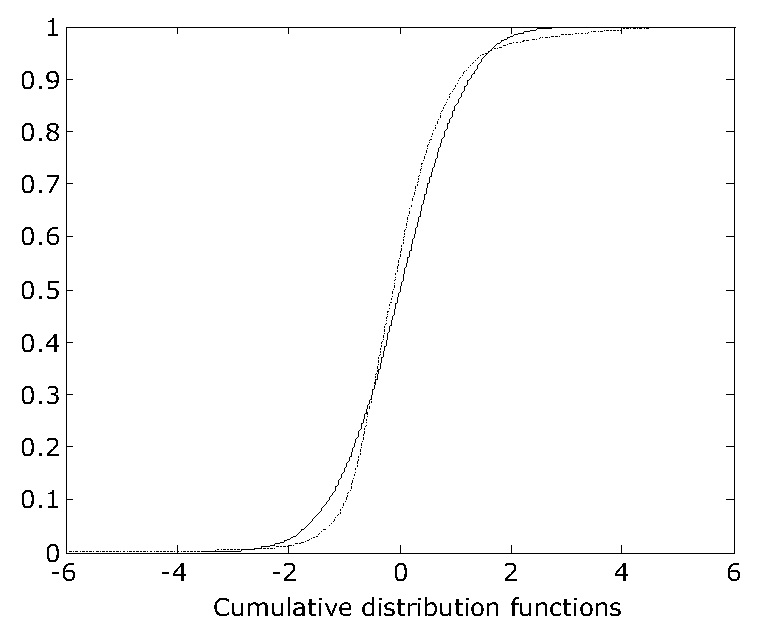
\includegraphics[width=0.40\textwidth]{figA1}
  \caption{Appendix figure.}
\end{figure}
\begin{table}[!h]
 \caption{Appendix table.}
 \begin{tabular}{|c|c|c|}
   \hline
   Algorithm & Performance [\%]& Calc. time [s]\\\hline\hline
   gradient & 95 & 100\\
   stochastic & 97 & 80\\
   evolutionary & 99 & 500\\\hline
 \end{tabular}
\end{table}

\begin{theorem}{}
\end{theorem}

\begin{lemma}{}
\end{lemma}

\begin{lemma}{}
\end{lemma}

\begin{lemma}{}
\end{lemma}
\end{appendices}

\begin{appendices}{}

\noindent This is another appendix,

\begin{equation}
  c=z+l.
\end{equation}

\begin{lemma}{Equivalence} Let us begin by ... xx xx  xxx xxx xxx xxx xxxxx xx xx xxxx xx xx xxx  xx xxx xxx xxx xx xx  xxx xxx xxx xxx xxxxx  xx xx xxxx xx xx xxx.
\end{lemma}

\end{appendices}

\makeinfo

\end{document}
